\subsection{1D model with TC PI theory}
\label{sec:1d-hurr}
To explore the impact that an increased amount of greenhouse gasses might have
on the system, consider a single layer model of the atmosphere (see Figure~\ref{fig:1d-atm}), described by the
set of four simultaneous equations.

\begin{figure}[htb!]
    \centering
    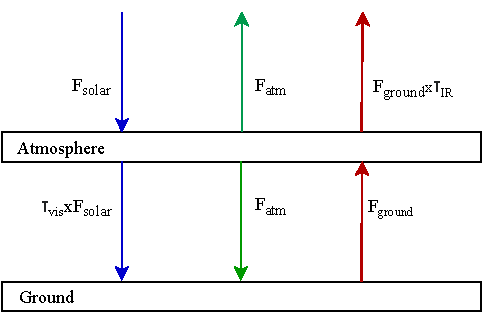
\includegraphics[width=0.7\linewidth]{images/two-level-model.pdf}
   \caption{The one level atmosphere model.}
    \label{fig:1d-atm}
\end{figure}


\begin{eqnarray}
F_{\mathrm{solar}} =& F_{\mathrm{atm}} + F_{\mathrm{ground}}\tau_{\mathrm{IR}}\\
F_{\mathrm{solar}}(1-\tau_{\mathrm{vis}}) =& 2F_{\mathrm{atm}} + F_{\mathrm{ground}}(\tau_{\mathrm{IR}}-1)\\
F_{\mathrm{ground}} = & F_{\mathrm{solar}}(\tau_{\mathrm{vis}}) +F_{\mathrm{atm}}  \\
F_{\mathrm{ground}} = & \sigma T_{\mathrm{ground}}{}^4 \\
F_{\mathrm{atm}} = & \sigma T_a{}^{4},
\end{eqnarray}

where F is the fluxes from the different areas of the model,
$ \tau_{\mathrm{IR}}$ and $\tau_{\mathrm{vis}}$ are the opacity of the atmosphere
to infrared and visible radiation respectively.
This leads to the solution

\begin{equation}
T_{\mathrm{ground}} = \left( \frac{F_{\mathrm{solar}}}{\sigma}\frac{(1+\tau_{\mathrm{vis}})}{(1+\tau_{\mathrm{IR}})}\right)^{1/4},
\end{equation}

which shows that when $\tau_{\mathrm{IR}}$, i.e.~the ammount of greenhouse gasses,
is increased, this leads to an increase in the temperature of the (sea) surface (c. $T_s$).
When using the Stefan-Boltzmann relation,

\begin{equation}
F_{\mathrm{atm}} = \sigma T_a{}^{4},
\end{equation}

we can further find that the

\begin{equation}
T_{\mathrm{atm}}^{4}=T_{\mathrm{ground}}^4\frac{(1-\tau_{\mathrm{vis}}\tau_{\mathrm{IR}})}{(1+\tau_{vis})}
\end{equation}

so that the temperature of the atmosphere (approximately equivalent to $T_{o}$)
decreases as the amount of greenhouse gases are increased.


One can then use,
\begin{equation}
\left|\mathbf{V}_{s}\right|^{2}=\frac{C_{k}}{C_{D}}
\frac{T_{s}-T_{o}}{T_{o}}\left(k_{0}^{*}-k\right),
\tag{PI}
\end{equation}

assuming that $\left(k_{0}^{*}-k\right)$ is constant then

\begin{align}
\frac{\left|\mathbf{V}_{s}\right|^{2}}{\left|\mathbf{V}_{s}\right|_{0}^{2}}
&=& \frac{T_{s}-T_{o}}{T_{o}}/\frac{T^{0}_{s}-T^{0}_{o}}{T^{0}_{o}}\\
&=& \frac{1- \left(\frac{1-\tau_{\mathrm{vis}}\tau_{\mathrm{IR}}}{1+\tau_{vis}}\right)^{-1/4}}
          {1- \left(\frac{1-\tau^{0}_{\mathrm{vis}}\tau^{0}_{\mathrm{IR}}}{1+\tau^{0}_{vis}}\right)^{-1/4}} &
\end{align}



 and see that as the numerator has increased, and the
denominator has decreased, the potential intensity is expected to increase with the
amount of greenhouse gases, $\tau_{\mathrm{IR}}$, in the atmosphere.
